\documentclass[12pt]{article}
\usepackage{multirow}
\usepackage{graphicx}
\usepackage{wrapfig}
\usepackage[T2A]{fontenc}			% кодировка
\usepackage[utf8]{inputenc}			% кодировка исходного текста
\usepackage[english,russian]{babel}	% локализация и переносы
\usepackage{amsmath,amsfonts,amssymb,amsthm,mathtools} 
\usepackage{hyperref}
\usepackage[rgb]{xcolor}
\usepackage{wasysym}
\usepackage{fancyhdr}
\pagestyle{fancy}
\usepackage[left=3cm,right=3cm, top=3cm, bottom=3cm, bindingoffset=0cm]{geometry}

\begin{document}
\begin{titlepage}
\begin{center}
\huge{Лабораторная работа № \textbf{4.6.2}}\\[1cm]\LARGE {Туннелирование миллиметровых радиоволн\\[7 cm]}
\end{center}

\begin{flushright}
\Large{Карманов Алексей\\752 группа}\\[9 cm]
\end{flushright}
\begin{center}
г.Долгопрудный\\
10.02.2019
\end{center}
\end{titlepage}
\fancyhead[L]
\indent \textbf{Цель работы:} экспериментальное исследование эффекта проникновения электромагнитных волн — туннелирования — через воздушный зазор между диэлектрическими призмами при полном внутреннем отражении на границе диэлектрик-воздух, а также моделирование интерферометра Майкельсона с использованием этого эффекта и измерение длины волны излучения и показателя преломления фторопласта для радиоволн миллиметрового диапазона.\\[0.75 cm]
\indent \textbf{В работе используются:} : генератор СВЧ-колебаний с рупорной антенной; приемная рупорная антенна и волновод; детектор; микроамперметр; металлические зеркала; две призмы и плоскопараллельная пластина из фторопласта; микрометрические винты.\\
\section{Теоретическая справка}
\subsection{Туннельный эффект}
В эксперименте мы наблюдаем туннелирование электромагнитной волны через узкую прослойку воздуха. Рассмотрим электромагнитную волну на границе раздела двух сред.\\
\begin{wrapfigure}{l}{0.5\textwidth}
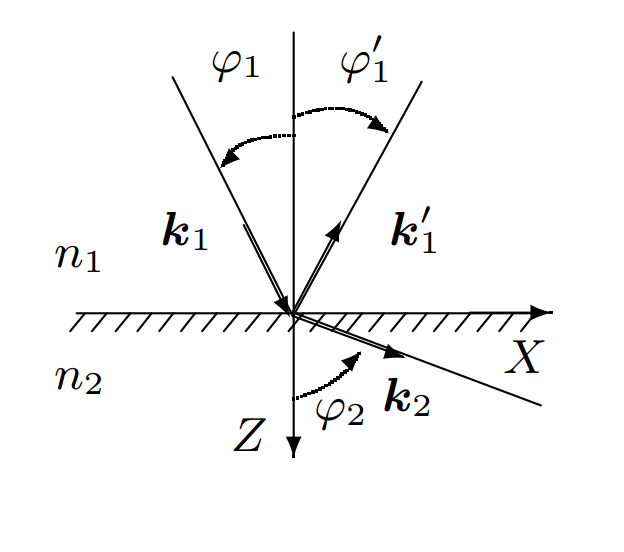
\includegraphics[width=0.55\textwidth]{teorborder}
\caption{Электромагнитная волна на границе раздела двух сред}
\end{wrapfigure}
Волновое уравнение формально допускает решения с мнимыми значениями $k_x$, $k_y$ или $k_z$. Такие волны также имеют реальный физический смысл и называются неоднородными в отличие от однородных плоских волн с действительными компонентами волнового вектора.\\
В качестве примера приведём волну с мнимым значением $k_z = \pm i \chi$:\\
\begin{equation}
\textbf{E} = \textbf{a}e^{\mp \chi z}e^{i(k_x x + k_y y)}e^{-i\omega t}. 
\end{equation}
Учтем граничные условия:
\begin{center}
$E_{1\tau} = E_{2\tau} \hspace{1 cm} D_{1n} = D_{2n}$ \\ 
$H_{1\tau} = H_{2\tau} \hspace{1 cm} B_{1n} = B_{2n}$  \\
\end{center}
Пусть $E_1$, $E`_1$ и $E_2$ — электрические поля в падающей, отражённой и преломлённой волнах соответственно:
\begin{equation}
E_1 = a_1 e^{ik_1(x sin{\phi_1} + z sin{\phi_1})}e^{-i\omega t};
\end{equation}
\begin{equation}
E`_1 = a`_1 e^{ik`_1(x sin{\phi`_1} + z sin{\phi`_1})}e^{-i\omega`_1 t};
\end{equation}
\begin{equation}
E_2 = a_2 e^{i(k_{2x}x + k_{2z}z)}e^{-i\omega_2 t}.
\end{equation}
.\\
При $\phi_1 > \phi_{\text{пр}} = arcsin(\frac{1}{n})$ волна во второй среде оказывается неоднородной и описывается выражением вида:
\begin{center}
$\textbf{E} = \textbf{a}e^{\mp \chi z}e^{i(k_x x + k_y y)}e^{-i\omega t}$
\end{center}, где $k_y = k_{2y} = 0, k_x = k_{2x} = k_1 sin\phi_1 $, а величина $\chi = \sqrt{k^2_1 sin^2\phi_1 - k_2^2}$.\\  [0.2 cm]
Таким образом, при $\phi_1 > \phi_{\text{пр}}$ электромагнитное поле во второй среде
(например, при переходе световой волны из стекла в воздух) экспоненциально затухает (или нарастает) с удалением от поверхности раздела. На основании закона сохранения энергии в выражении вида (1) перед положительной величиной $\chi$ следует брать знак – , соответствующий затухающей волне.\\ [0.2 cm]
Экспоненциальную функцию, описывающую затухание волны с удалением от поверхности раздела, удобно записать в виде $exp(-z/2\Lambda)$, где $\Lambda = \frac{1}{2\chi}$. Тогда интенсивность волны, пропорциональная квадрату амплитуды, изменяется с расстоянием по закону\\
\begin{equation}
 I \propto e^{-z/\Lambda}.
\end{equation} 
Длина затухания $\Lambda$ может быть представлена выражением:
\begin{equation}
\Lambda = \frac{\lambda_2}{4\pi\sqrt{n^2 sin^2\phi_1 - 1}}
\end{equation}
\section{Экспериментальная установка}
Туннелирование миллиметровых радиоволн через тонкий воздушный зазор переменной толщины изучается на установке, схема которой приведена на рис. 2. Источником радиоволн является высокочастотный генератор Г4-115 на трёх отражательных клистронах, перекрывающих полосу частот от 25,80 ГГц до 37,50 ГГц, разделённую на три поддиапазона. Генерирующий при выбранной настройке клистрон возбуждает в прямоугольном металлическом волноводе сечением 7,2 x 3,4 $мм^2$ электромагнитную волну, которая распространяется вдоль волновода и с помощью рупорной антенны $А_1$ излучается в пространство. Задача антенны заключается в том, чтобы сделать излучение более направленным. Электрический вектор волны, бегущей вдоль волновода и излучаемый антенной, перпендикулярен широкой стенке волновода. На пути радиоволн устанавливаются две одинаковые прямые призмы $П_1$ и $П_2$ с почти прямоугольным (рис. 1) равнобедренным треугольником в основании. Уменьшение угла при вершине треугольника на $16^\circ$ сделано для устранения обратных отражений. Призмы изготовлены из фторопласта, обладающего малыми потерями на высоких радиочастотах. Узкие грани призм ограничивают воздушную прослойку, ширина которой может изменяться с помощью микрометрических винтов $M_1$ и $M_2$.
\begin{figure}
\begin{center}
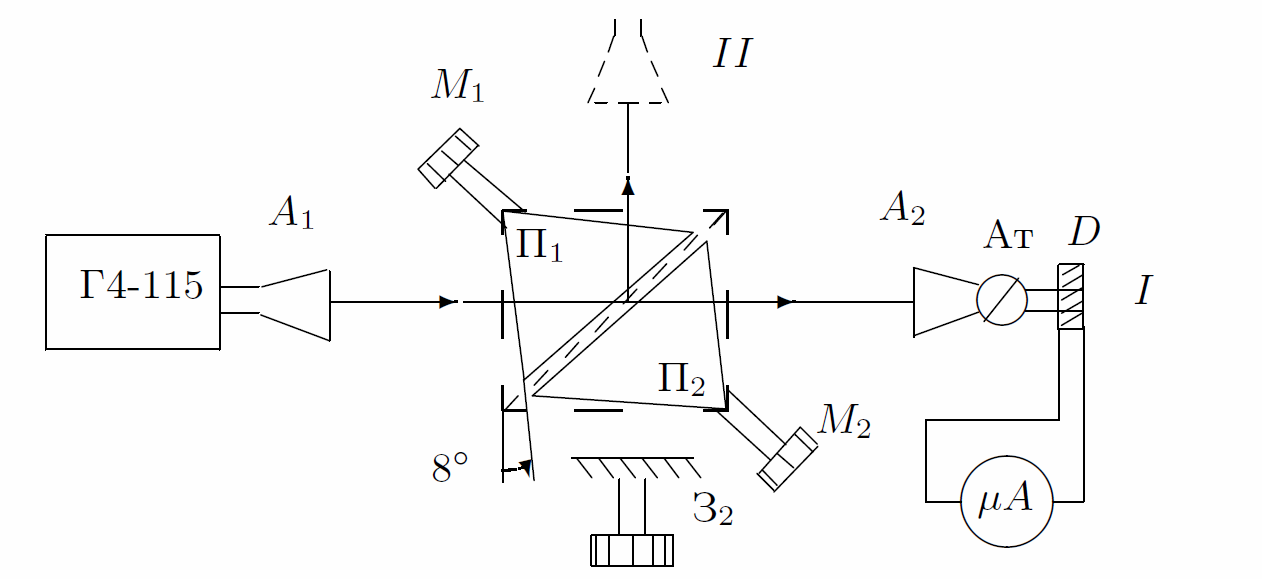
\includegraphics[width=0.8\textwidth]{tunnelteor}
\caption{установка для исследования туннельного эффекта}
\end{center}

\end{figure}


Для измерения показателя преломления материала призм интерференционным методом перед неподвижным зеркалом устанавливается пластина известной толщины $h$ из того же материала, что и призмы фторопласта. В этом плече интерферометра возникает приращение длины "оптического" пути. Это приращение можно скомпенсировать, передвинув подвижное зеркало на необходимое расстояние $\delta x$. Показатель преломления определяется из условия для $\delta x$.
\begin{figure}[!h]
\begin{center}
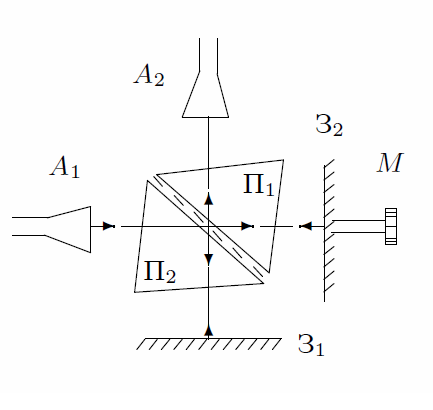
\includegraphics[width=0.5\textwidth]{interferometrteor}
\caption{интерферометр Мейкельсона}
\end{center}
\end{figure}
\section{Исследование туннелирования радиоволн}
1. Проведем настройку аппаратуры для проведения измерения показателя преломления фторопласта с помощью метода исследования туннельного эффекта .\\
2. Снимем зависимость интенсивности прошедшей волны от величины воздушного зазора. Результаты занесем в Таблицу 1.\\
3. Переставим приёмник для измерения отраженного сигнала и снимем зависимость интенсивности отраженной волны от величины воздушного зазора.\\
4. Построим график зависимости коэффициентов T и R от величины воздушного зазора и убедимся, что T + R = 1.\\

\begin{table}[!h]
\caption{Показатели сигнала приемника в зависимости от ширины зазора}
\begin{tabular}{|l|l|l|l|l|l|l|l|l|l|l|l|l|}
\hline
\multicolumn{2}{|l|}{l, мм}&  6.0 & 6.5 & 7.0 & 7.5 & 8.0 & 8.5 & 9.0 & 9.5 & 10.0 & 10.5 & 11.0 \\ \hline
\multirow{2}{*}{J, мА}& Пройденная& 8.5 & 8.5 & 8.5 & 7.8 & 6.5 & 5.3 & 4.5 & 3.7 & 2.7 & 2.0 & 1.4 \\ \cline{2-13} 
                      & Отраженная & 0 & 0 & 0 & 1.8 & 2.0 & 3.1 & 4.3 & 5.3 & 6.3 & 7.1 & 8.1  \\ \hline
\end{tabular}
\end{table}
\begin{figure}[!h]
\begin{center}
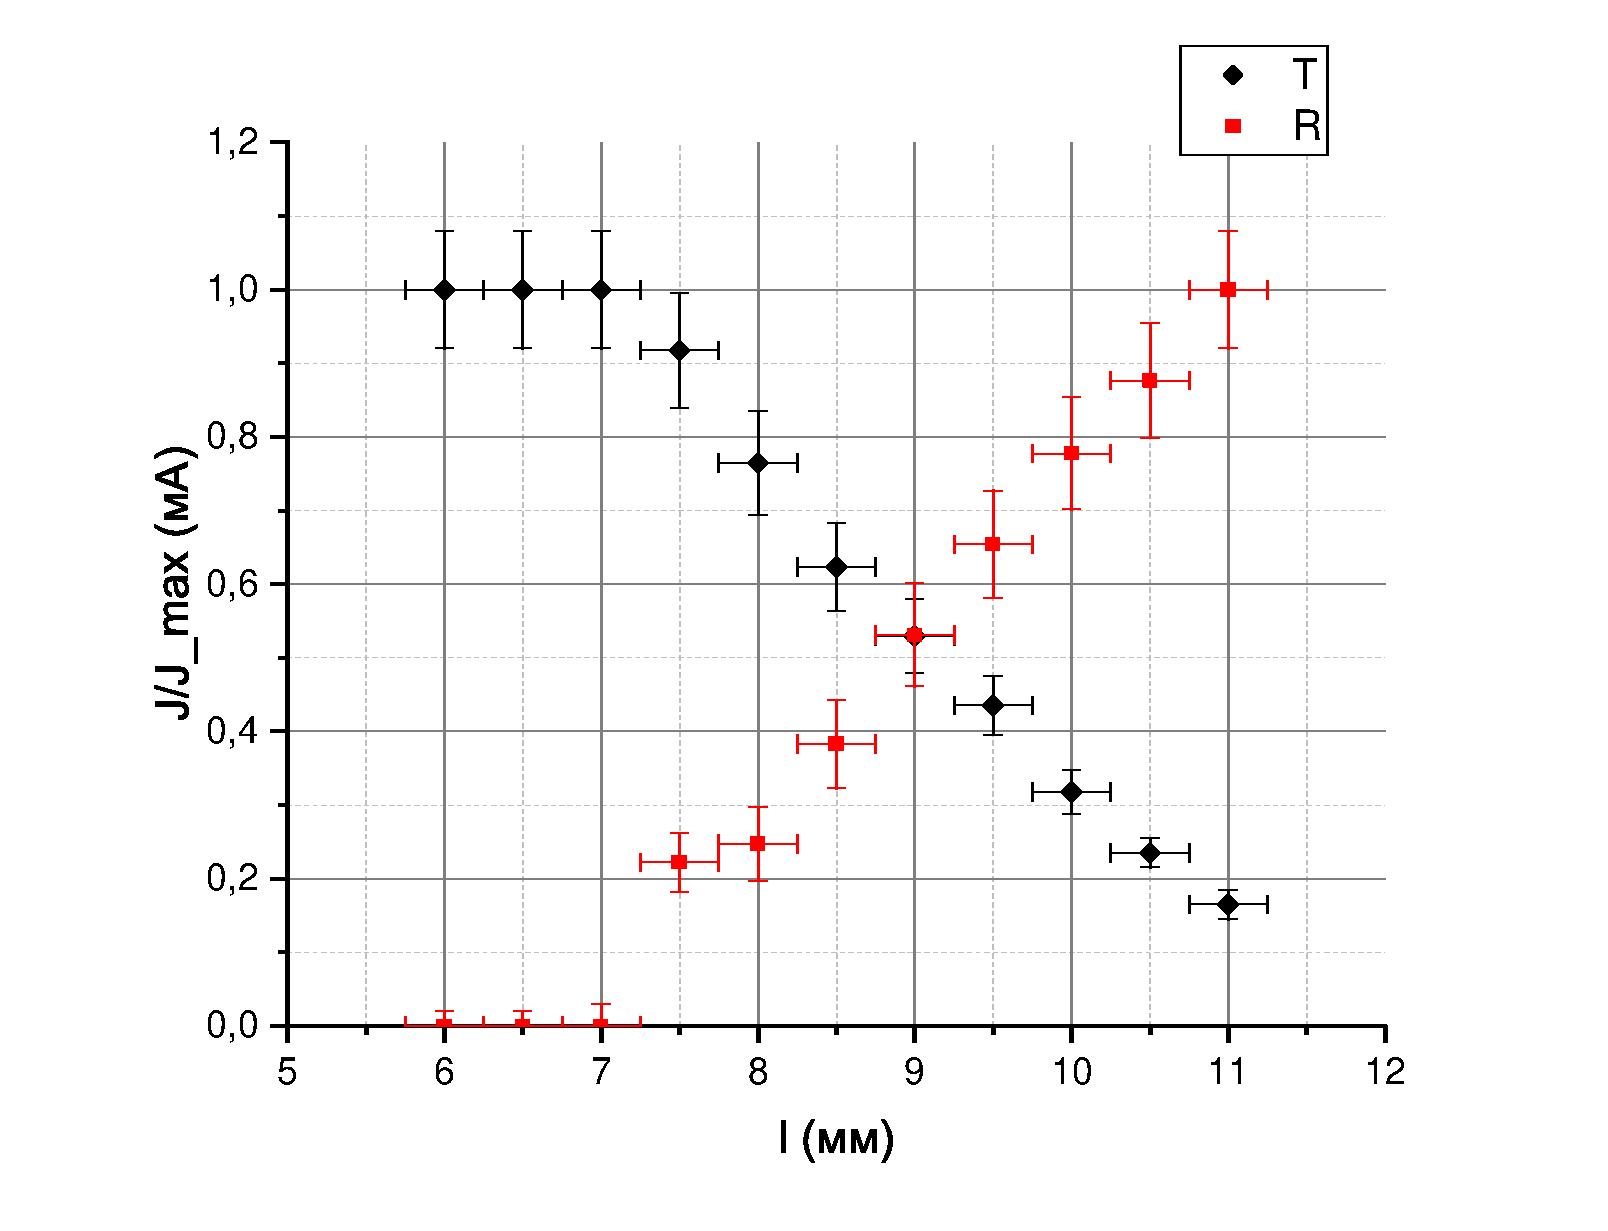
\includegraphics[width = 0.92\textwidth]{TplusR}
\caption{Прошедшяя T и отраженная R волны}
\end{center}
\end{figure}
\newpage
5. Теперь построем график зависимости $ln(T)$ от показаний микрометра $z$.\\ По наклону прямой посчитаем оценим длину затухания $\Lambda$, а затем - показатель преломления хлоропласта.\\
\begin{figure}[!h]
\begin{center}
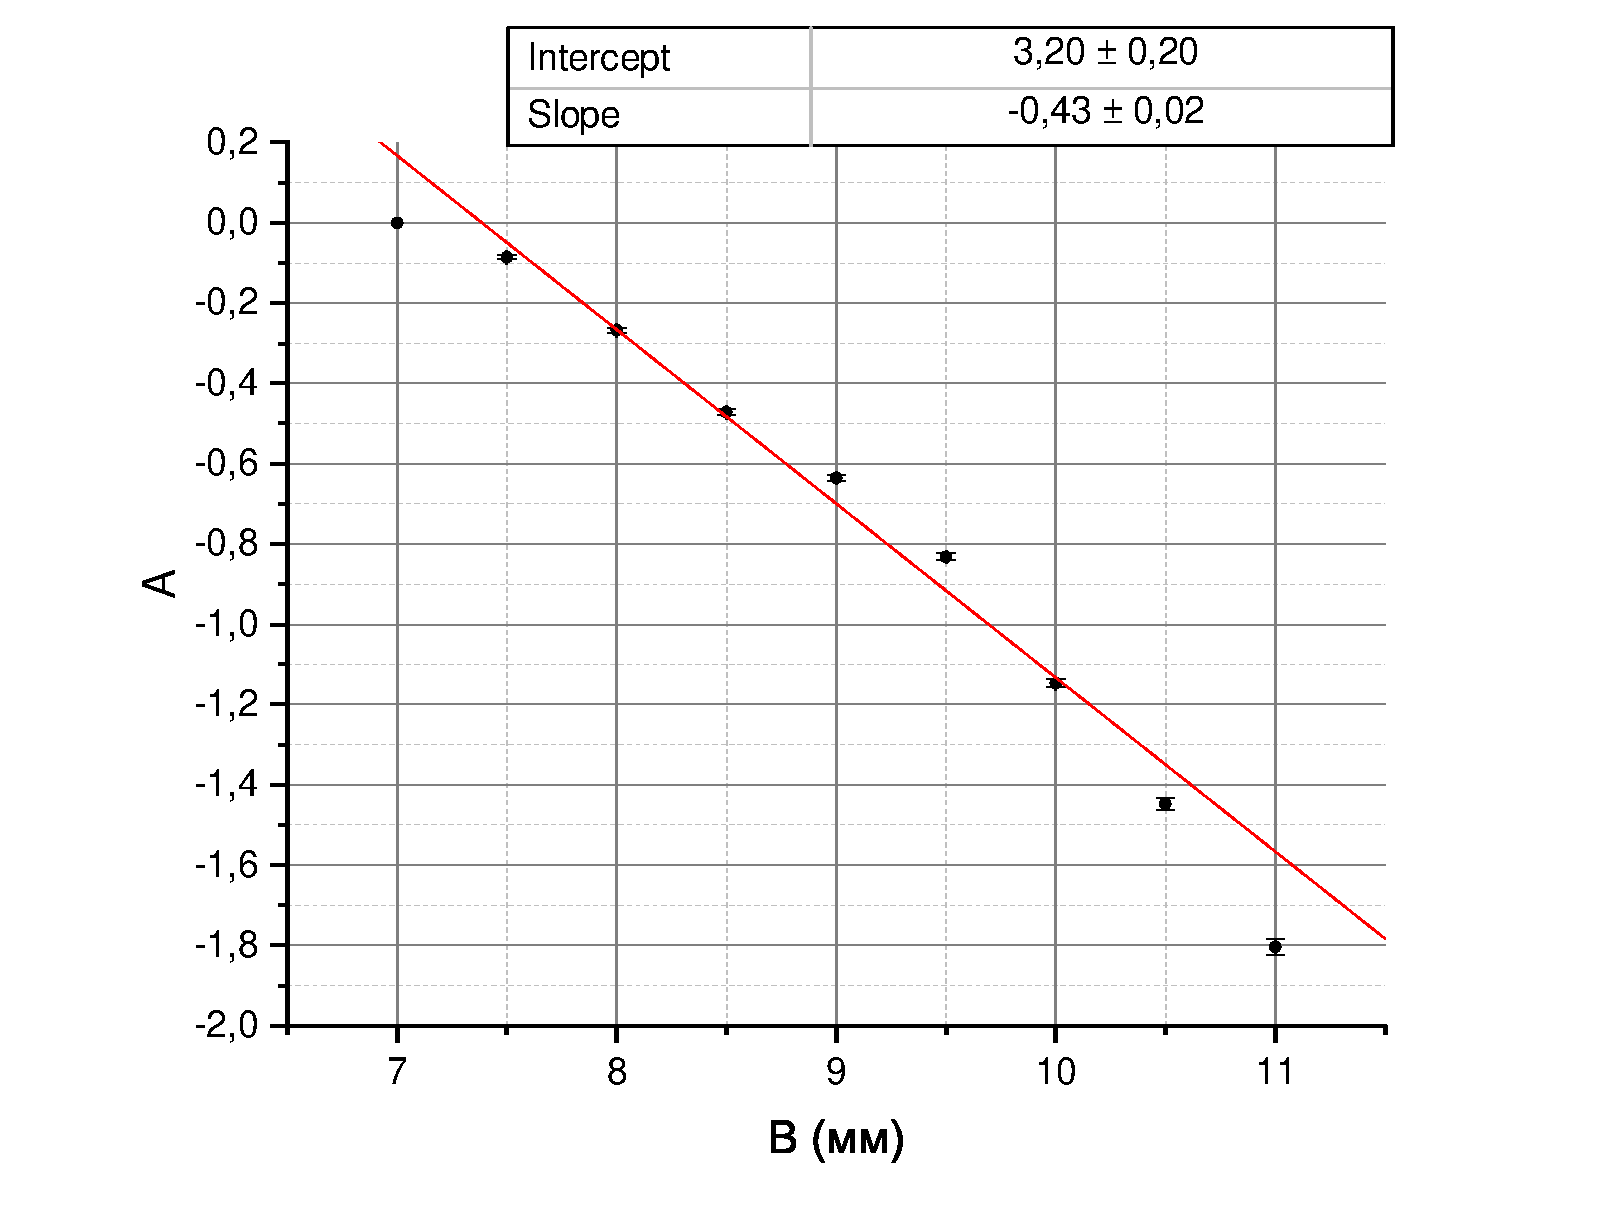
\includegraphics[width = \textwidth]{lnT}
\caption{зависимости $ln(t)$ от показаний $z$}
\end{center}
\end{figure}
Из наклона прямой получили значение длины затухания: $\Lambda = 2,3 \pm 0,3$ мм.\\
Теперь расчитаем показатель преломления фторопласта: $n = 1,41 \pm 0,15$\\
\newpage
\section{Интерферометр Майкельсона}
1. Соберем модель интерферометра Майкельсона.\\
2. Снимем зависимость тока от координаты подвижного зеркала и по графику определим длину волны радиоволн:\\
\begin{table}[!h]
\caption{Зависиомсть сигнала на приемнике от положения зеркала}
\begin{center}

\begin{tabular}{|l|l|l|l|l|l|l|l|l|}
\hline
l, мм  & 50 & 51 & 52 & 52.5 & 53 & 53.5 & 54 & 55 \\ \hline
J, мА & 0.2 & 0.3 & 3.2 & 4.0 & 4.1 & 2.2 & 0.8 & 0.1 \\ \hline

\end{tabular}

\end{center}
\end{table}
\begin{figure}[!h]
\begin{center}
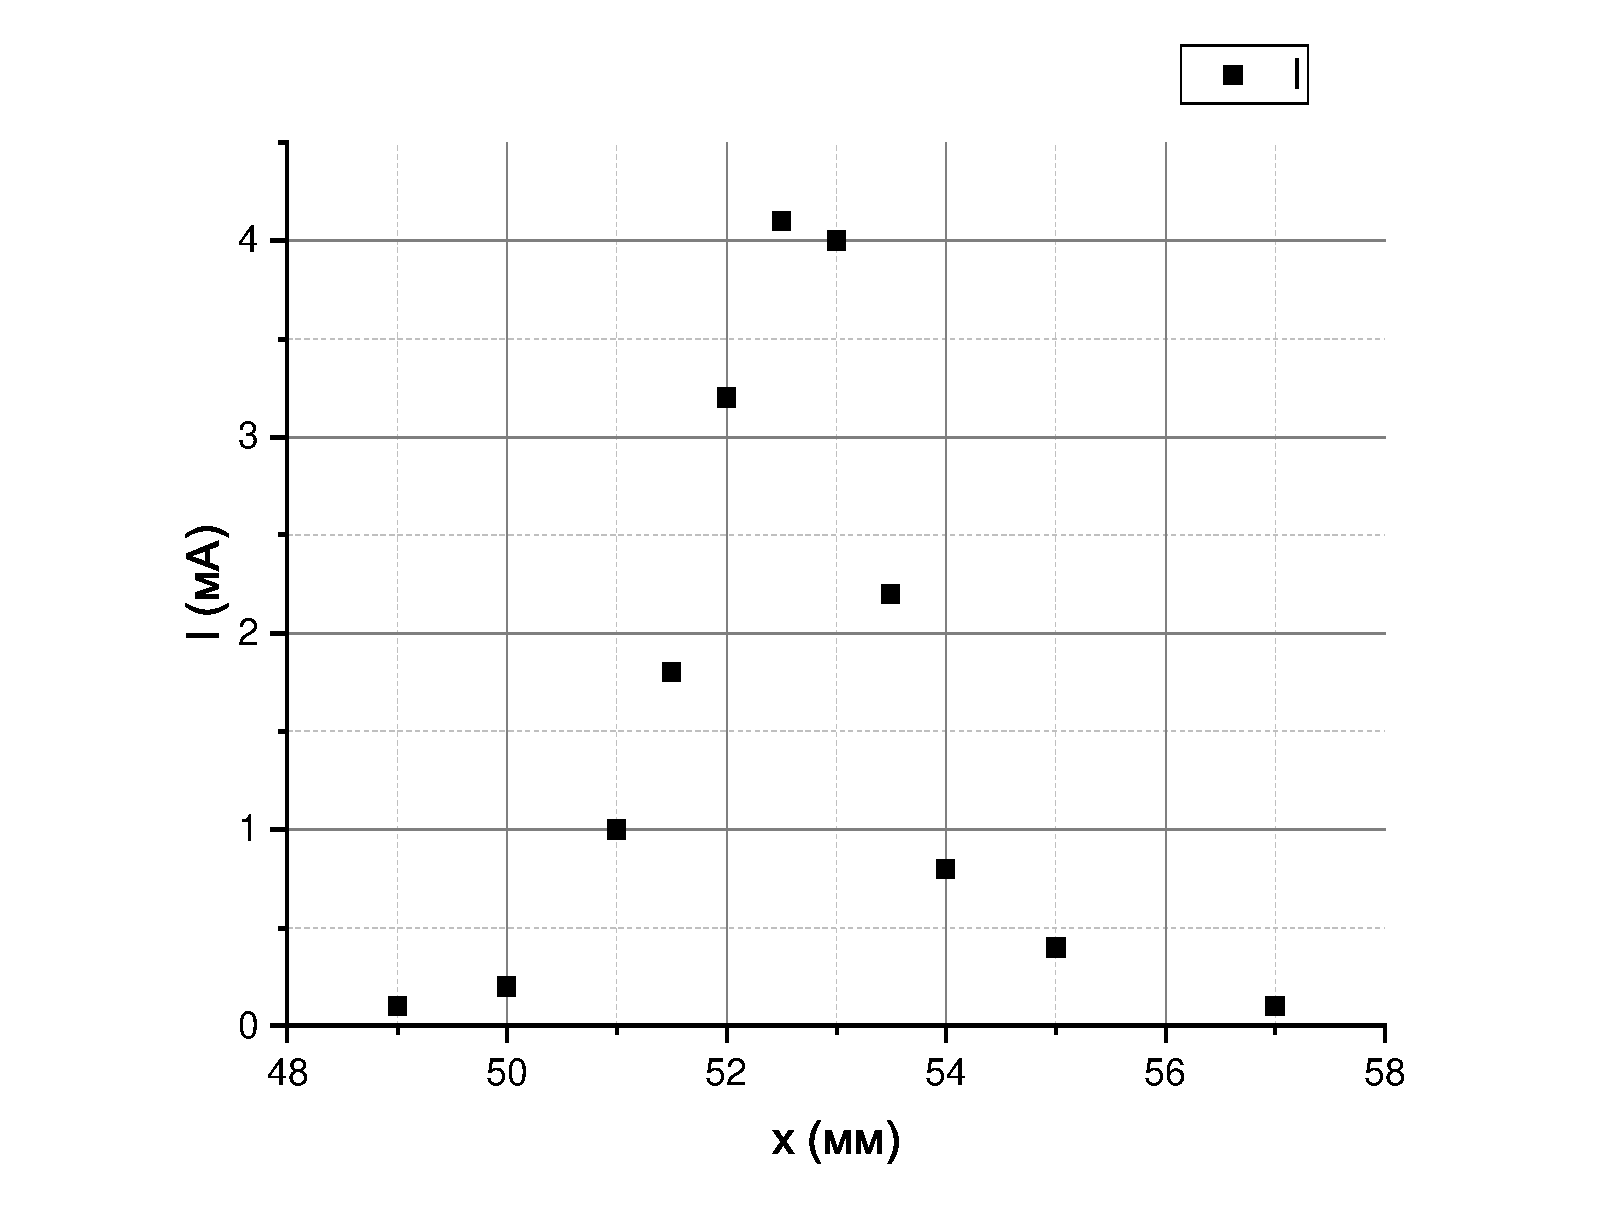
\includegraphics[width = 0.85\textwidth]{interf}
\caption{Интерференционная картина}
\end{center}
\end{figure}
Экспериментально определенная длина волны примерно равна $\lambda_0 \approx 7$ мм.\\
3. Настроим интерферометр на максимум, вставим образец фторопласта толщиной $h = 6,2$ мм, после - скомпенсируем изменение длины. Расчитаем показатель преломления фторопласта интерференционным методом:\\
\begin{center}
$n = 1,45 \pm 0,12$
\end{center} 
\end{document}